\section{Introduzione}

%=======================================================================

\begin{frame}{Obiettivi del lavoro di tirocinio}

\begin{itemize}[<+->]
    \item Metti gli obiettivi
\end{itemize}

\end{frame}

%=======================================================================

\begin{frame}{Tecnologie utilizzate}

\begin{columns}
    \begin{column}{0.5\textwidth}
        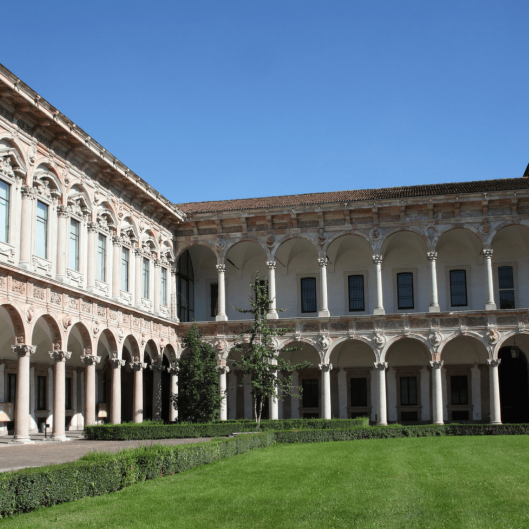
\includegraphics[width=0.5\textwidth]{assets/background_alternative.png}
    \end{column}
    \begin{column}{0.5\textwidth}
        \begin{block}{Titolo}
            Roba
        \end{block}
    \end{column}
\end{columns}

\end{frame}

%=======================================================================

\begin{frame}{Processo di standardizzazione}

    \setupchronology{startyear=2017,stopyear=2024,color=maincolor,startdate=false,stopdate=false}
    \setupchronoperiode{teststyle=\it,startdate=false,stopdate=false,textdepth=-0.5cm}
    \setupchronoevent{textstyle=\it,year=false,markdepth=0.3cm}
    \setupchronograduation[event]{markdepth=1.5cm}
    
    \startchronology
        \chronograduation{1}
        \chronoevent{2018}{Inizio}
        \chronoperiode[color=red]{2018}{2019}{Raccolta}
        \chronoevent{2019}{Round 1}
        \chronoperiode[color=yellow]{2019}{2021}{Round 2}
        \chronoperiode[color=green]{2021}{2023}{Finale}
        \chronoevent{2023}{Standardizzazione}
    \stopchronology

\end{frame}

%=======================================================================

\begin{frame}{Famiglia ASCON}
    Le tre famiglie
\end{frame}
